%
% File emnlp2020.tex
%
%% Based on the style files for ACL 2020, which were
%% Based on the style files for ACL 2018, NAACL 2018/19, which were
%% Based on the style files for ACL-2015, with some improvements
%%  taken from the NAACL-2016 style
%% Based on the style files for ACL-2014, which were, in turn,
%% based on ACL-2013, ACL-2012, ACL-2011, ACL-2010, ACL-IJCNLP-2009,
%% EACL-2009, IJCNLP-2008...
%% Based on the style files for EACL 2006 by 
%%e.agirre@ehu.es or Sergi.Balari@uab.es
%% and that of ACL 08 by Joakim Nivre and Noah Smith

\documentclass[11pt,a4paper]{article}
\usepackage[hyperref]{emnlp2020}
\usepackage{times,latexsym}
\usepackage{url}
\usepackage[T1]{fontenc}
\usepackage{graphicx}
\usepackage{algorithm}
\usepackage{algorithmic}
\usepackage[leftcaption]{sidecap}
\sidecaptionvpos{figure}{t}
\usepackage{amsmath}
\usepackage{amsfonts}
\usepackage{amsthm}
\usepackage{todonotes}
\newcommand{\eref}[1]{Eqn.\ (\ref{#1})}  % Eqn
\newcommand{\sref}[1]{Sec.\ \ref{#1}}    % Section
\newcommand{\figref}[1]{Fig.\ \ref{#1}}  % Figure
\newcommand{\tabref}[1]{Table \ref{#1}} % Table
\newcommand{\algref}[1]{Algorithm \ref{#1}} % Algorithm
\newcommand{\prg}[1]{\noindent\textbf{#1}} %Paragraph
\newcommand{\KL}[2]{\ensuremath{KL\left({#1}\, \| \, {#2}\right)}}
\usepackage{amssymb}
 \usepackage{multirow}
 \usepackage[normalem]{ulem}


\usepackage{tabularx}
%\newcolumntype{L}{>{\centering\arraybackslash}m{3cm}}

\newtheorem{lemma}{Lemma}

\definecolor{Green}{RGB}{50,200,50}
\newcommand{\ndg}[1]{\textcolor{Green}{[ndg: #1]}}
\newcommand{\dorsa}[1]{\textcolor{magenta}{[dorsa: #1]}}
\newcommand{\rdh}[1]{\textcolor{blue}{[rdh: #1]}}
\newcommand{\minae}[1]{\textcolor{orange}{[minae: #1]}}
\renewcommand{\thefigure}{S\arabic{figure}}
\renewcommand{\thetable}{S\arabic{table}}

\renewcommand{\UrlFont}{\ttfamily\small}

% This is not strictly necessary, and may be commented out,
% but it will improve the layout of the manuscript,
% and will typically save some space.
\usepackage{microtype}

%\aclfinalcopy % Uncomment this line for the final submission
%\def\aclpaperid{***} %  Enter the acl Paper ID here

%\setlength\titlebox{5cm}
% You can expand the titlebox if you need extra space
% to show all the authors. Please do not make the titlebox
% smaller than 5cm (the original size); we will check this
% in the camera-ready version and ask you to change it back.

\newcommand\BibTeX{B\textsc{ib}\TeX}

\title{Supplemental Materials for \\ Continual Adaptation for Efficient Machine Communication}

\author{First Author \\
  Affiliation / Address line 1 \\
  Affiliation / Address line 2 \\
  Affiliation / Address line 3 \\
  \texttt{email@domain} \\\And
  Second Author \\
  Affiliation / Address line 1 \\
  Affiliation / Address line 2 \\
  Affiliation / Address line 3 \\
  \texttt{email@domain} \\}

\date{}

\begin{document}
\maketitle

\begin{figure*}
\centering
\includegraphics[scale=0.9]{../figures/examples.pdf}
\caption{Complete set of referring expressions produced by (A) a \emph{human speaker} interacting with our listener model and (B) our \emph{speaker model} interacting with a human partner, as described below in Appendix D. Utterances are color-coded with the response accuracy. Green is correct; red is incorrect.}
\label{fig:examples}
\end{figure*}

\section*{Appendix A: derivation of incremental KL}

We denote the distribution over a sequence of $T$ tokens by $p(w_{1:T}) = p(w_1, w_2, \dots, w_T)$.
We are interested in the KL divergence between two such distributions, $\KL{p(w_{1:T})}{q(w_{1:T})}$.
We show that our approximation over possible captions is the best incremental estimator of this intractable objective. 
First, note that the KL divergence factors in the following way.


\begin{lemma}
\begin{equation*}
\begin{split}
& \KL{p(w_{1:2})}{q(w_{1:2})}  \\
& = \, \KL{p(w_1)}{q(w_1)} \\
 & \quad + \mathbb{E}_{p(w_1)} \KL{p(w_2 | w_1)}{q(w_2 | w_1)}\\
 \end{split}
\end{equation*}
%where
%\begin{equation*}
%f_{p,q}(t_1,t_2) = 
%\end{equation*}
\end{lemma}
\begin{proof}
\phantom\qedhere
\begin{equation*}
\begin{split}
& \KL{p(w_{1:2})}{q(w_{1:2})} \\
& = \sum_{w_1}\sum_{w_2}p(w_{1:2})\log\frac{p(w_{1:2})}{q(w_{1:2})} \\
& =   \sum_{w_1}\sum_{w_2}p(w_{1:2})\log\frac{p(w_1)}{q(w_1)}  \\
 &\quad + \sum_{w_1}\sum_{w_2}p(w_{1:2})\log\frac{p(w_2|w_1)}{q(w_2|w_1)} \\
 & = \sum_{w_1}\log\frac{p(w_1)}{q(w_1)}\sum_{w_2}p(w_{1:2}) \\
 &\quad + \sum_{w_1}p(w_1)\sum_{w_2}p(w_2 | w_1)\log\frac{p(w_2|w_1)}{q(w_2|w_1)} \\
 & = \KL{p(w_1)}{q(w_1)} \\
 & \quad + \mathbb{E}_{p(w_1)} \KL{p(w_2 | w_1)}{q(w_2 | w_1)}
\end{split}
\end{equation*}
\end{proof}

Now, let $w^{*}_1$ be the token at which $p(w_1)$ takes its maximum value.
Then $w^{*}_1$ is the best single-sample approximation of the expectation:
\begin{equation*}
\begin{split}
& \mathbb{E}_{p(w_1)} \KL{p(w_2 | w_1)}{q(w_2 | w_1)} \\
& \approx \KL{p(w_2 | w^{*}_1)}{q(w_2|w^{*}_1}\\
\end{split}
\end{equation*}
If we assume that $p(w_{1:T})$ is Markov (as in a recurrent model) then it follows from repeatedly applying the lemma that
\begin{equation*}
\begin{split}
& \KL{p(w_{1:T})}{q(w_{1:T})} \\
& = \sum_{i=1}^T \KL{p(w_i | w^{*}_1, \dots, w^*_{i-1})}{q(w_i|w^*_1\dots, w^*_{i-1}}\\
& = \sum_{i=1}^T \KL{p(w_i | w^*_{i-1})}{q(w_i | w^*_{i-1})}
\end{split}
\end{equation*}
recovering our objective.

%\begin{figure*}[h!]
%\centering
%\includegraphics[scale=0.75]{../figures/speaker-model-examples.pdf}
%\caption{ Even when the initial caption is incorrect about details (e.g. the woman in the bottom row is holding a sandwich, not cake), the human listener was able to determine which one was intended in context, allowing the model to update its expectations and successfully use ``cake'' on later repetitions.}
%\label{fig:speakermodelexamples}
%\end{figure*}

\section*{Appendix B: Parameter settings}

For both the speaker task and listener task, we used a learning rate of 0.0005, took 6 gradient steps after each trial, and used a batch size of 8 when sampling utterances from the augmented set of sub-phrases, 
At each gradient step, we sampled 50 objects from the full domain $\mathcal{O}$ of COCO to approximate our regularization term.
We set the coefficients weighting each term in our loss function as follows: 1.0 (utterance loss), 0.1 (contrastive loss), 0.5 (KL regularization), 0.3 (local rehearsal).


 \begin{figure*}[t!]
\centering
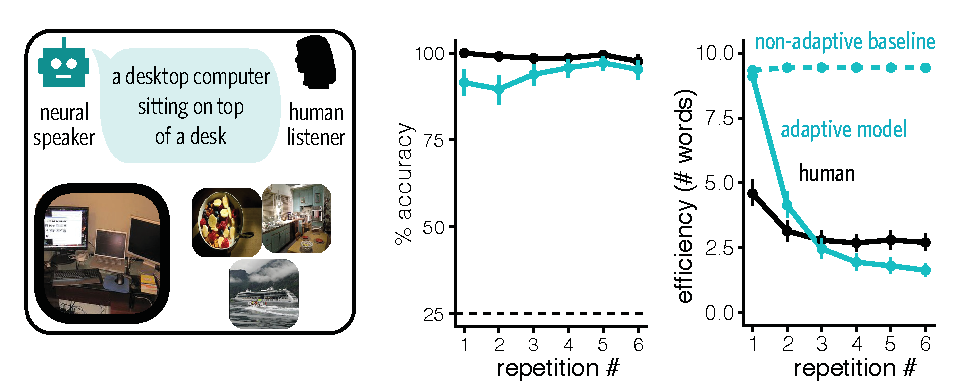
\includegraphics[scale=0.9]{../figures/supplementalCurves_conll}
\caption{Speaker model evaluations with human listener. Error ribbons are bootstrapped 95\% CIs.}
\label{fig:supplementalcurves}
\end{figure*}

\section*{Appendix C: Regression details}

To formally test increasess in efficiency reported for baseline pairs of humans in Sec.~4.1 (see Fig. 3 and \ref{fig:supplementalcurves}), we conducted a mixed-effects regression predicting utterance length. 
We included a fixed effect for context type (i.e. `simple' vs. `challenging') as well as orthogonalized linear and quadratic effects of repetition number, and each of their interactions with context type. 
We also included random intercepts accounting for variability in initial utterance length at the pair- and image-level.
To test increases in the adaptive listener model's accuracy in Sec.\ 4.2, we conducted a mixed-effects logistic regression on trial-level responses (i.e. `correct' vs. `incorrect') with the same effect structure, removing context type, as this experiment was only conducted on challenging contexts.
This same effect structure was used to test improvements in the adaptive speaker model's efficiency in Sec.~4.3. 

We tested our listener ablations in Sec.\ 5.2 using a mixed-effects logistic regression with fixed effects of repetition number and model variant, as well as participant-level random intercepts and slopes (for repetition number). We dummy-coded the models setting the baseline at the full model, to facilitate direct comparison. 


\section*{Appendix D: Speaker evaluation and analysis}

\subsection*{Task description}

We designed the speaking task such that the pre-trained model's \emph{efficiency} --- the number of words needed to identify the target --- would be poor at the outset. 
Because the COCO captions seen during pre-training were relatively exhaustive (i.e.~mentioning many attributes of the image), we required \emph{simple} contexts where the pre-trained model would produce more complex referring expressions than required to distinguish the images. 
To construct simple contexts we sampled images randomly from different COCO category labels.
For example, one context might contain an image of an elephant, an image of a boat, and so on.

\subsection*{Evaluation results}
\label{sec:speaking_task}

We evaluated our model in the \emph{speaking} task using simple contexts, which requires the model to form more efficient conventions given feedback from human responses.
53 participants from Amazon Mechanical Turk were paired to play the listener role with our speaker model.
Utterances were selected from the LSTM decoder using beam search with a beam width of 50 and standard length normalization to mitigate the default bias against long utterances \cite[e.g.][]{wu2016google}.
After producing an utterance, the model received feedback about the listener's selection. 
If its partner correctly selected the intended target, it proceeded to adapt conditioning on the new observation; in the event of an incorrect response, it refrained from updating.
This strategy thus only leads to inferences about utterance meanings (and sub-phrase meanings, through data augmentation) after positive evidence of understanding.

As expected, the model starts with much longer captions than human speakers use in simple contexts (Fig.\ \ref{fig:supplementalcurves}).
It uses nearly as many words for simple contexts as humans used for challenging contexts. 
However, it gets dramatically more efficient over interaction while maintaining high accuracy. 
We found a significant decrease in utterance length over successive repetitions, $t=35,~p <0.001$, using the same mixed-effects regression structure reported above.
A non-adapting baseline shows no improvement, as it has no mechanism for changing its expectations about utterances over time.

\begin{table*}[h!]
\resizebox{\textwidth}{!}{%
\begin{tabular}{p{4cm} | p{3.5cm} | p{3cm} | p{2.7cm} | p{1.6cm} | p{1.3cm}}
Rep.~1 & Rep.~2 & Rep.~3 & Rep.~4 & Rep.~5 & Rep.~6 \\
\hline
a group of people standing on a sandy beach & a group of people standing on top        & a group of people standing          & a group of people & a group of & a group  \\
\hline
a couple of zebra standing next to trees    & a couple of zebra standing next          & a couple of zebra                   & a couple of       & a couple   & a couple \\
\hline
a living room filled with lots of furniture & a living room filled with lots furniture & a living room filled with furniture & a living room     & a living   & a living
\end{tabular}%
}
\caption{Examples of utterances produced by ablated speaker with pure cost penalty instead of data augmentation, which quickly become ungrammatical and incoherent.}
\label{tab:badbad_examples}
\end{table*}


\subsection*{Pragmatic reasoning supports speaker informativity}
\label{sec:pragmatic_analysis}



We now proceed to analyze the \emph{speaking task}, beginning with the role of pragmatic reasoning.
In principle, incorporating pragmatic reasoning during adaptation (i.e. in our contrastive likelihood term) introduces an inductive bias for \emph{mutual exclusivity} \cite{SmithGoodmanFrank13_RecursivePragmaticReasoningNIPS, FrankGoodmanTenenbaum09_Wurwur,gandhi2019mutual}.
When the listener correctly selects the target, the speaker not only learns that the listener believes this is a good description for the target but can also infer that the listener \emph{does not} think it is a good description for the other objects in context; otherwise, they would have selected one of the other objects instead.
Thus, in addition to boosting listener adaptation, we expected explicit pragmatic reasoning to allow the speaker to gradually produce more informative, distinguishing utterances. 

The \emph{challenging} contexts provide an ideal setting for evaluating speaker pragmatics, because the pre-trained speaker model initially produces the same caption for all four images in context.
We simulated games with our adaptive speaker as well as an ablated variant with no contrastive term in its adaptation objective.
The model was always given feedback that the correct target was selected.
We measured informativity by examining the proportion of words that overlapped between the utterances produced for the different images in a particular context: $|u_i \cap u_j| / \min(|u_i|, |u_j|)$ for combinations of utterances ($u_i,u_j$) where $i \neq j$. 
This measure ranges between 0\% when the intersection is empty and 100\% in the event of total overlap. 

Even though both the full model and the ablated variant initially produce completely overlapping utterances, we found a rapid differentiation of utterances for the model with pragmatics intact, as each image becomes associated with a distinct label.
Meanwhile, the ablated version continues to have high overlap even on later repetitions: it often ends up producing the same one-word label for multiple objects as it reduces (Fig.\ \ref{fig:speakerablation}A).

 \begin{figure}[b!]
\centering
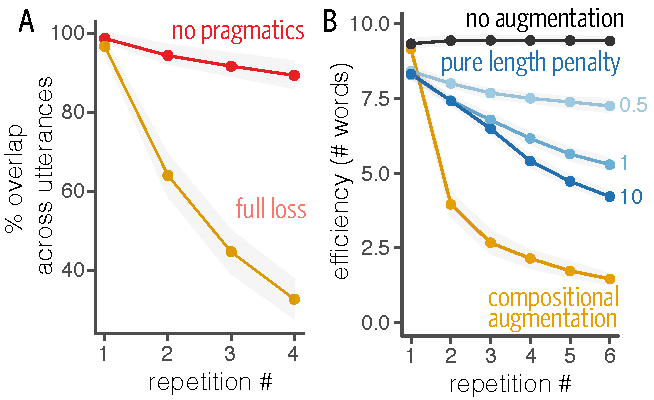
\includegraphics[scale=0.7]{../figures/lossComparisonResults.pdf}
\vspace{-2em}
\caption{Speaker model ablations. (A) The contrastive loss allows the model to become informative in challenging contexts. (B) Compositionally augmenting adaptation data with sub-phrases of the utterance allows stronger gains in efficiency than a simple length penalty. Error ribbons are bootstrapped 95\% CIs.}
\vspace{-.5em}
\label{fig:speakerablation}
\end{figure}

\subsection*{Compositional data augmentation supports efficiency}
%
Finally, we investigated the role played by the compositional data augmentation mechanism for allowing our speaker model to become more efficient (Fig.\ \ref{fig:speakerablation}B).
Two concerns may be raised about this mechanism.
First, it is possible that the RNN decoder architecture is already able to appropriately update expectations about sub-parts from the whole without being given explicit parses, so augmentation is redundant. 
Second, it may be argued that this augmentation mechanism just imposes a glorified length penalty \emph{forcing} the speaker to shorten, rather than allowing efficiency to come out of the model naturally.

To address these concerns, we compare augmentation with two variants: (1) an ablated model with no augmentation, and (2) an alternative mechanism that explicitly imposes a length cost at production time. 
This alternative is implemented by re-ranking the top 25 utterances from beam search according to $U(u_i) = P(u_i)/\ell(w) - \beta_w \ell(w)$ where the first term is the length-normalized beam-search objective and the second term is an explicit bias for shorter utterances.
When $\beta_w=0$, this is equivalent to top-$k$ beam search but as $\beta_k \rightarrow \infty$, the model will increasingly prefer short utterances.

We simulated the behavior of these model variants in each of the 53 games we collected in our interactive speaking task, using the same sequence of images and feedback about correctness. 
We found that that the ablated model with no augmentation fails to become more efficient: at least for our RNN decoder architecture, evidence of success only reinforces expectations about the full caption; it cannot not propagate this evidence to the individual parts of the utterance.
A sufficiently high length penalty does allow utterances to become shorter, but reduces linearly rather than quadratically (as humans do; \citealp{ClarkWilkesGibbs86_ReferringCollaborative,hawkins2019characterizing}).
Moreover, upon inspecting the utterances produced by this variant (see Table \ref{tab:badbad_examples}), we found that it simply cuts off the ends of utterances, whereas compositional data augmentation is based on a syntactic parse and thus allows the model to preserve grammaticality and gradually build expectations about meaningful sub-units.
In sum, we find that our augmentation mechanism is not reducible to a coarse length bias, and is able to compensate for representation failures in current recurrent architectures \cite{dasgupta2018evaluating, nikolaus2019compositional}.\footnote{We expect that a more structured architecture, able to propagate evidence about the meaning of a full utterance to representations of intermediate semantic units, would make this augmentation step redundant \cite[e.g.][]{tai2015improved,gan2017semantic,mccoy_does_2020}.}


\bibliographystyle{acl_natbib}
\bibliography{../references.bib}

\end{document}
